\clearpage
\newpage
% also set appendices to new page
%\addtocontents{toc}{\protect\newpage} #todo to shift appendix in toc on new page
\appendix      %is not resetting counters?
\section*{Appendix}
\addcontentsline{toc}{section}{Appendix}
\addtocontents{toc}{\protect\addtolength{\protect\cftsubsecnumwidth}{10pt}} % form here on add space in toc between number and name of section must be increased, because of roman numrals
\renewcommand\thesubsection{A.\Roman{subsection}}

% redefine names for floats (prepend A.)
\renewcommand\thefigure{A.\arabic{figure}}   
\renewcommand\thetable{A.\arabic{table}}
\renewcommand\thelstlisting{A.\arabic{lstlisting}} 
% reset counters
\setcounter{figure}{0}                        
\setcounter{table}{0}
\setcounter{lstlisting}{0} 

\subsection{Persisting Issues of STEGO}\label{subsec:stego-persisting-issued}
\begin{itemize}
    \item The hardcoded properties of default datasets should instead be placed in configuration files.
    This is a design issue and does not influence results.
    \item When executing the evaluation procedure, the comparison with \gls{picie}~\autocite{Cho2021} is not possible (a class not found error is thrown).
    This is because of implementation flaws that cannot be fixed easily, but is only relevant for this comparison.
    \item A benign RuntimeWarning concerning the C header of numpy is issued by Cython, which is usually silenced in the numpy-init function, but silencing happens do be removed in the numpy version in the \gls{stego} environment. Since the environment could not be altered, this warning is just ignored. For more details on this warning see the discussion on github~\autocite{rgommers2012}.
    %".../lib/python3.6/importlib/_bootstrap.py:219: RuntimeWarning: numpy.ufunc size changed, may indicate binary incompatibility. Expected 192 from C header, got 216 from PyObject"
    % no problem: https://stackoverflow.com/questions/40845304/runtimewarning-numpy-dtype-size-changed-may-indicate-binary-incompatibility
    \item DDP warnings are issued ``Grad strides do not match bucket size''.
    This may only impair performance, but not results.
    \item A torch warning is issued because ``compute method'' is called before ``update method''.
    Since the compute method is only called to tell \tensorboard{} to monitor this metric in the future, this is not a problem.
    \item CropComputer class should not be a dataset, but get and adjust a dataset.
    This is a design issue and does not influence results.
\end{itemize}

\clearpage

\clearpage
\subsection{Screws Predictions with Pre-trained Models}
\begin{figure}[!htb]
    \centering
    \includegraphics[clip,trim={0 0 0 36}, height=\textwidth, angle=90]{pictures/experiment_1/pretrained-models_cluster-predictions_example_predictions_2_all}\\
    \caption[Predictions from Provided Models]{Predictions from provided models. Visualisation of image, ground truth, raw cluster predictions and clusters combined by most likely match to ground truth label. Raw cluster colors correspond to cluster names in~\autoref{fig:correlation-matrix-pretrained}. All shown slices belong to volume syn009HG and are ordered according to spatial location in the volume. Every 100th slice is shown. Image rotated by 90~degree.}
    \label{fig:pretrained-predictions_syn009}
\end{figure}
\clearpage

\subsection{Cross-validation of Screws Data Set}\label{subsec:cross-validation-screws}
\begin{table}[!htb]
    \centering
    \makegapedcells
    \begin{tabular}{|c|p{0.62\textwidth}|p{0.2\textwidth}|}
        \hline
        \textbf{Fold} & \textbf{Train set} &\textbf{Validation~set} \\
        \hline
        0 & 113731Mg10, syn018, syn020, syn021, syn022, syn026, syn030, syn032, syn033, syn038, syn041 & 113724Mg10, 113726Mg5, 113728Mg10 \\
        \hline
        1 & 113724Mg10, 113726Mg5, 113728Mg10, syn021, syn022, syn026, syn030, syn032, syn033, syn038, syn041 & 113731Mg10, syn018, syn020 \\
        \hline
        2 & 113724Mg10, 113726Mg5, 113728Mg10, 113731Mg10, syn018, syn020, syn030, syn032, syn033, syn038, syn041 & syn021, syn022, syn026 \\
        \hline
        3 & 113724Mg10, 113726Mg5, 113728Mg10, 113731Mg10, syn018, syn020, syn021, syn022, syn026, syn038, syn041 & syn030, syn032, syn033 \\
        \hline
        4 & 113724Mg10, 113726Mg5, 113728Mg10, 113731Mg10, syn018, syn020, syn021, syn022, syn026, syn030, syn032, syn033 & syn038, syn041 \\
        \hline
        \hline
        {\small LOO} 1 & 113731Mg10, 113724Mg10, 113728Mg10, syn018, syn020, syn021, syn022, syn026, syn030, syn032, syn033, syn038, syn041 & 113726Mg5 \\
        \hline
        {LOO} 2 &  113731Mg10, 113724Mg10, 113726Mg5, syn018, syn020, syn021, syn022, syn026, syn030, syn032, syn033, syn038, syn041& 113728Mg10\\
        \hline
        {LOO} 3 &  113724Mg10, 113726Mg5, 113728Mg10, syn018, syn020, syn021, syn022, syn026, syn030, syn032, syn033, syn038, syn041 &  113731Mg10\\
        \hline
        { LOO 4} & 113731Mg10, 113724Mg10, 113726Mg5, 113728Mg10,syn020, syn021, syn022, syn026, syn030, syn032, syn033, syn038, syn041 &  syn018\\
        \hline
        { LOO 5} &   113724Mg10, 113726Mg5, 113728Mg10, 113731Mg10, syn018, syn021, syn022, syn026, syn030, syn032, syn033, syn038, syn041 & syn020\\
        \hline
        %\makecell{\textbf{Test set}\\\textbf{Exp. 1}} & \multicolumn{2}{c|}{113734HQMg5, syn009HQ, 113729HQMg5} \\
        %\hline
    \end{tabular}
    \caption[Cross-validation Sets of Screws Data Set]{Cross-validation sets of screws data set. For each fold volumes names for train and validation set are given. Folds of the leave-one-out cross-validation are marked with ``LOO'' to indicate difference from the five-fold cross-validation folds.} % Since the number of volumes is not a multiple of 5 the last fold of the five-fold cross-validations only contains two volumes in the validation set. 
    \label{tab:folds-screws}
\end{table}

\clearpage
\subsection{Parameters Used for Training}
\begin{table}[!htb]
    \centering
    \makegapedcells
    \begin{tabular}{|c|r|>{\raggedleft\arraybackslash}p{0.19\textwidth}|>{\raggedleft\arraybackslash}p{0.19\textwidth}|}
        \hline
        \makecell{\textbf{Parameter}} & \makecell{\textbf{Base-case,}\\ \textbf{extra clusters}} & \makecell{\textbf{Random} \\ \textbf{cropped} \\ \textbf{(200~px)}} & \makecell{\textbf{Random} \\ \textbf {cropped} \\ \textbf{(96~px)}} \\
        \hline
        \makecell{ $\lambda_{rand}$ \\ neg\_inter\_weight} & 0.4 & 0.4 & 0.4 \\ \hline
        \makecell{ $\lambda_{knn}$ \\pos\_inter\_weight} & 0.2 & 0.2 & 0.2 \\ \hline
        \makecell{ $\lambda_{self}$ \\pos\_intra\_weight} & 0.4 & 0.4 & 0.4 \\ \hline
        \makecell{$b_{rand}$\\neg\_inter\_shift} & 0.85 & 0.55 & 0.5 \\ \hline
        \makecell{$b_{knn}$\\pos\_inter\_shift} & 0.45 & 0.45 & 0.4 \\ \hline
        \makecell{$b_{self}$\\pos\_intra\_shift} & 0.35 & 0.35 & 0.55 \\ \hline
    \end{tabular}
    \caption[Training Parameters]{Parameters Used for Training. For each of the trainings the six manually selected parameters are given. Each parameter is named by their configuration file name as well as the corresponding name in \gls{stego} paper. Parameters where tuned according to recommendations from \gls{stego}s authors, with minor changes, as explained in~\autoref{subsubsec:discussion-experiment2}.}
    \label{tab:training-parameters}
\end{table}


\clearpage
\subsection{Runtimes of Experiments}
\begin{table}[!htb]
\centering
\makegapedcells
\begin{tabular}{|l|l|r|}
    \hline
    \textbf{Experiment} & \textbf{Description} & \textbf{Runtime} \\
    \hline
    Exp. 1 & Prediction with Potsdam model & $\approx$ 5.25~hours\\ \hline
    Exp. 1 & Prediction with Cocostuff model & $\approx$ 11.75~hours\\ \hline
    Exp. 1 & Prediction with Cityscapes model & $\approx$ 12.25~hours\\ \hline
    \hline
    Exp. 2 & \makecell[l]{Train base-case\\batch size: 8} & $\approx$1.25~days\\ \hline
    Exp. 2 & \makecell[l]{Train extra clusters\\batch size: 8} & $\approx$1.25~days\\ \hline
    Exp. 2 & \makecell[l]{Train random cropped (200~px)\\batch size: 16} & $\approx$4.5~hours\\ \hline
    Exp. 2 & \makecell[l]{Train random cropped (96~px)\\batch size: 32} & $\approx$1.5~hours\\ \hline
    Exp. 2 & \makecell[l]{Train base-case leave one out\\batch size: 8} & $\approx$1.5~days\\ \hline
\end{tabular}
\caption[Runtimes of Experiments]{Runtimes of experiments. Each experiment was run on a computation node, containing four V100 GPUs. For the predictions total run time is given. For the trainings approximate runtime for one fold and the batch size is given.}
\label{tab:runtimes}
\end{table}

\clearpage
\subsection{Fold- and Label-wise Development of IoU}
\begin{figure}[!htb]
    \centering
    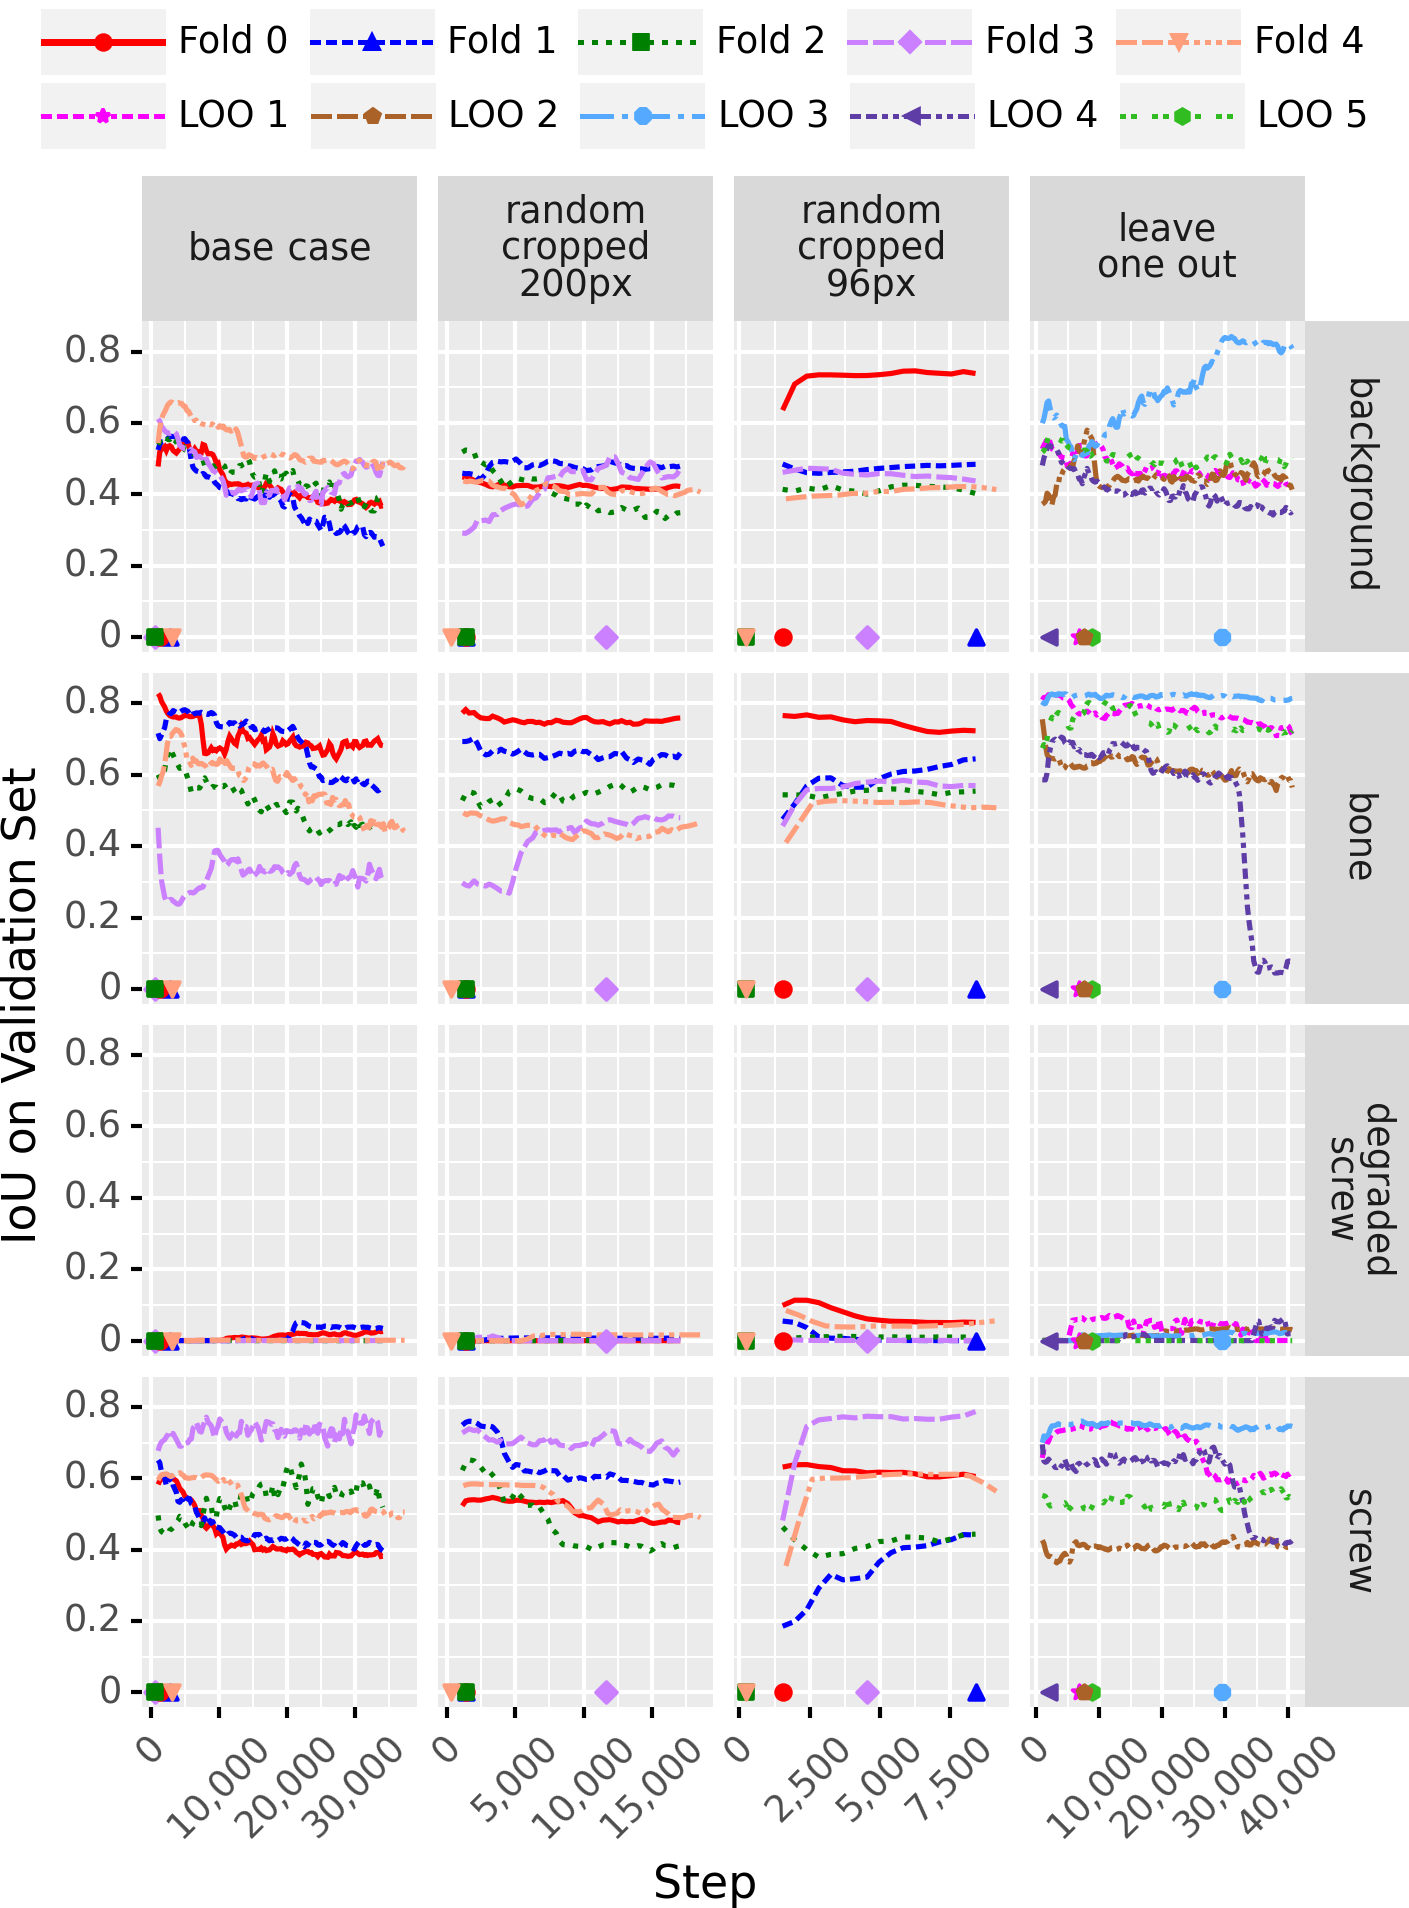
\includegraphics[width=\textwidth]{pictures/experiment_2/mIoU_labels_folds_separate_base-case_final_base-case_loo_random_cropped_final_random_cropped_res96_final}\\
    \caption[Fold- and Label-wise Development of IoU]{Fold- and label-wise development of IoU. For each cross-validation the moving average (over three data points) of the IoU per label and fold is displayed. So the first three data points are not depicted in the plots. Additionally, on the x-axis the step number of the best overall model per fold (in terms of mIoU) is marked.}
    \label{fig:miou-per-fold-label}
\end{figure}

\clearpage
\subsection{Fold-wise Development of Accuracy}
\begin{figure}[!hb]
    \centering  %trim={<left> <lower> <right> <upper>}
    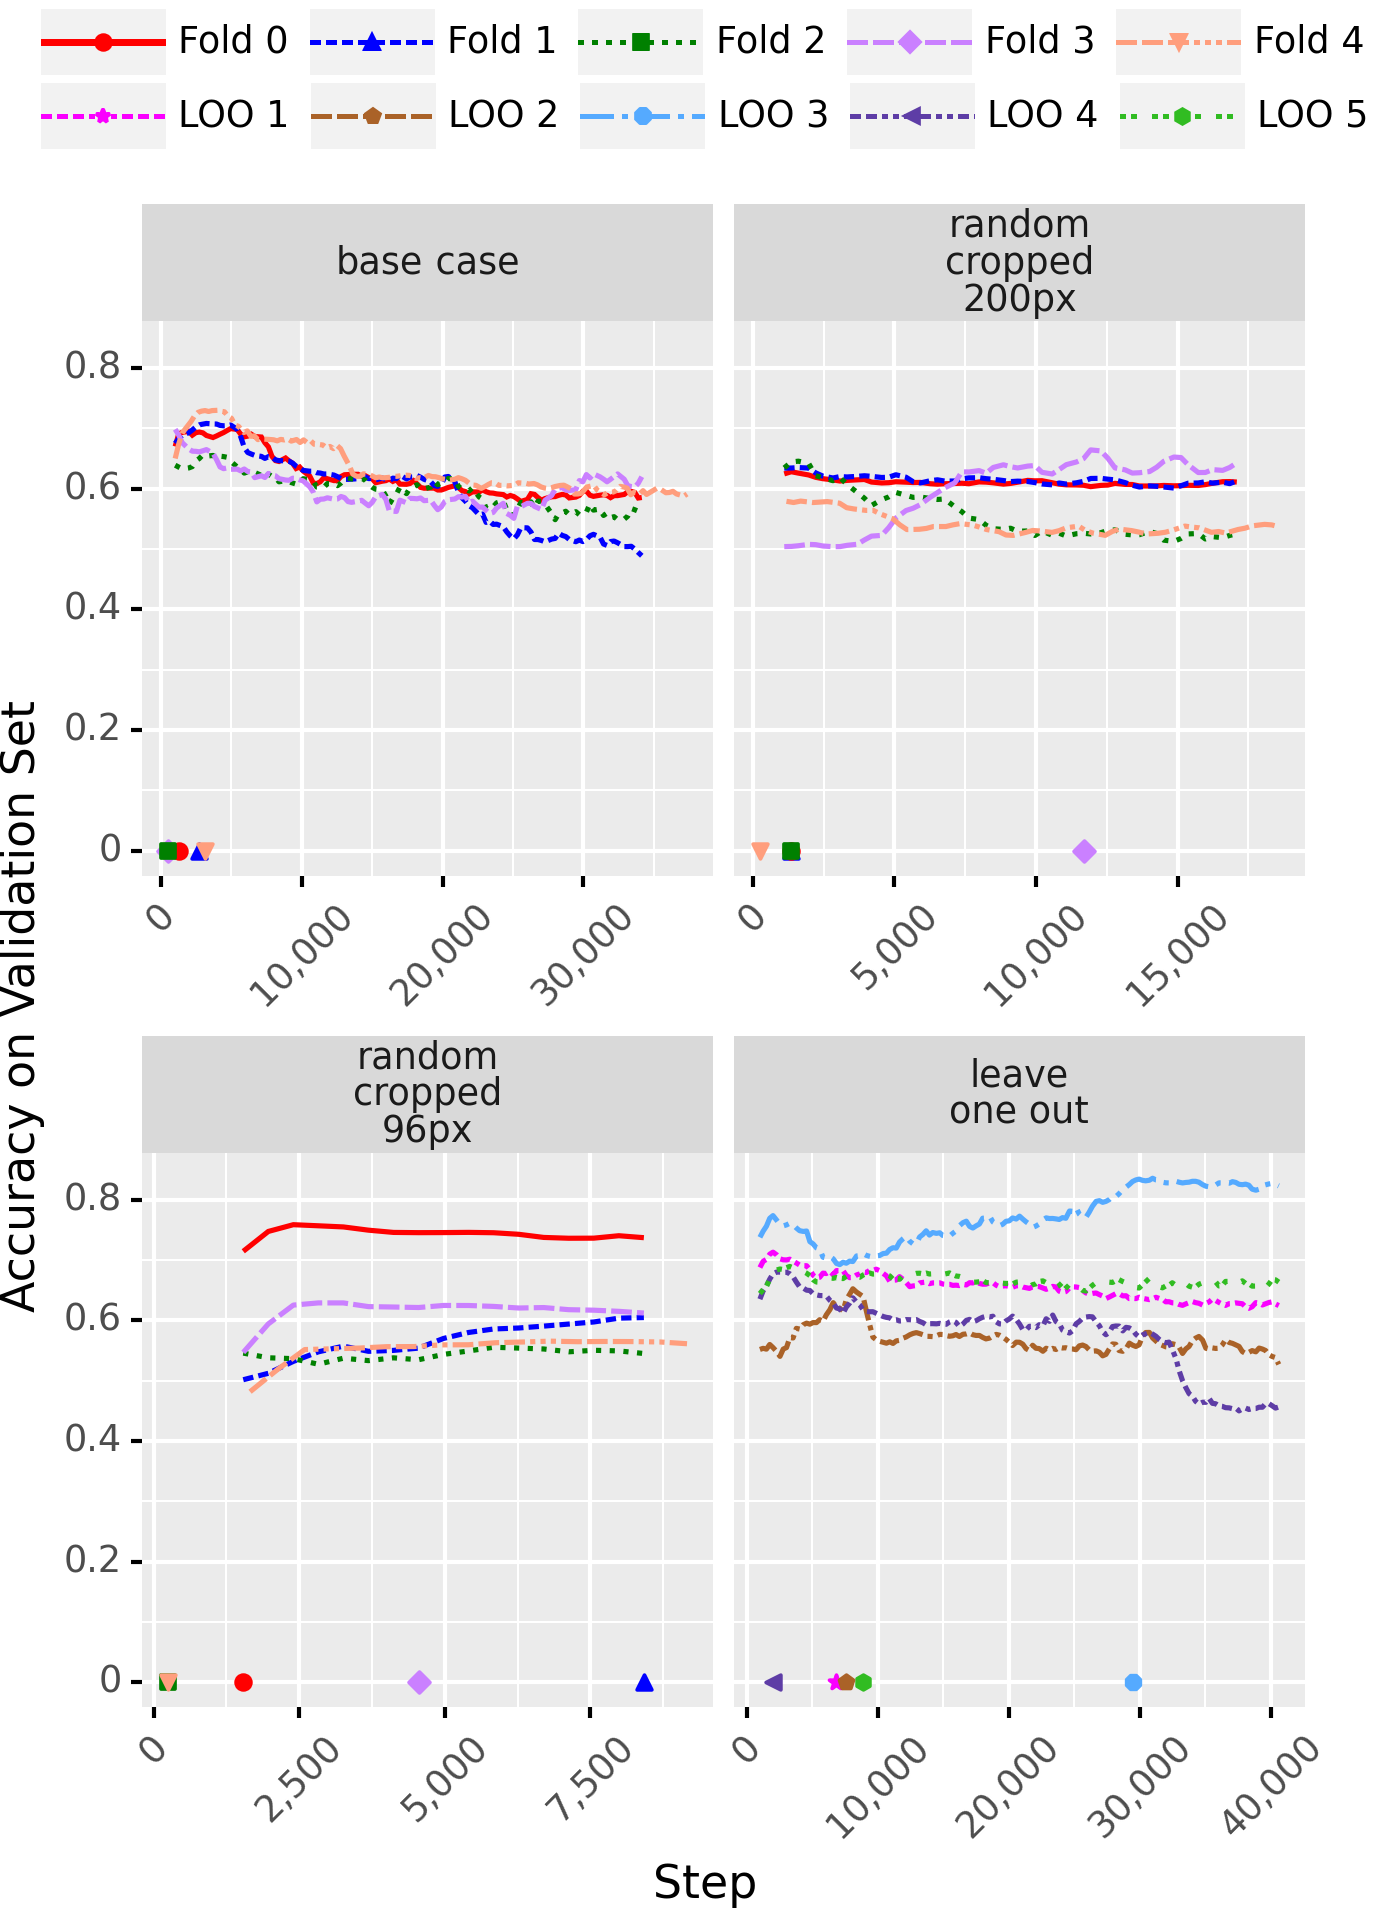
\includegraphics[width=0.95\textwidth]{pictures/experiment_2/accuracy_base-case_final_base-case_loo_random_cropped_final_random_cropped_res96_final}\\
    \caption[Fold-wise Development of Accuracy]{Fold-wise development of Accuracy. For each cross-validation the moving average (over three data points) of the Accuracy per fold is displayed. So the first three data points are not depicted in the plots. Additionally, on the x-axis the step number of the best overall model per fold (in terms of mIoU) is marked. Note, that Accuracy takes nearly the same course as mIoU just shifted upwards. }
    \label{fig:accuracy-per-fold}
\end{figure}

\clearpage
\subsection{Example Predictions for Trained Models}\label{subsec:example-predictions-for-cropping-regimes}
\begin{figure}[!htb]
    \centering      
                            %<left> <lower> <right> <upper>
    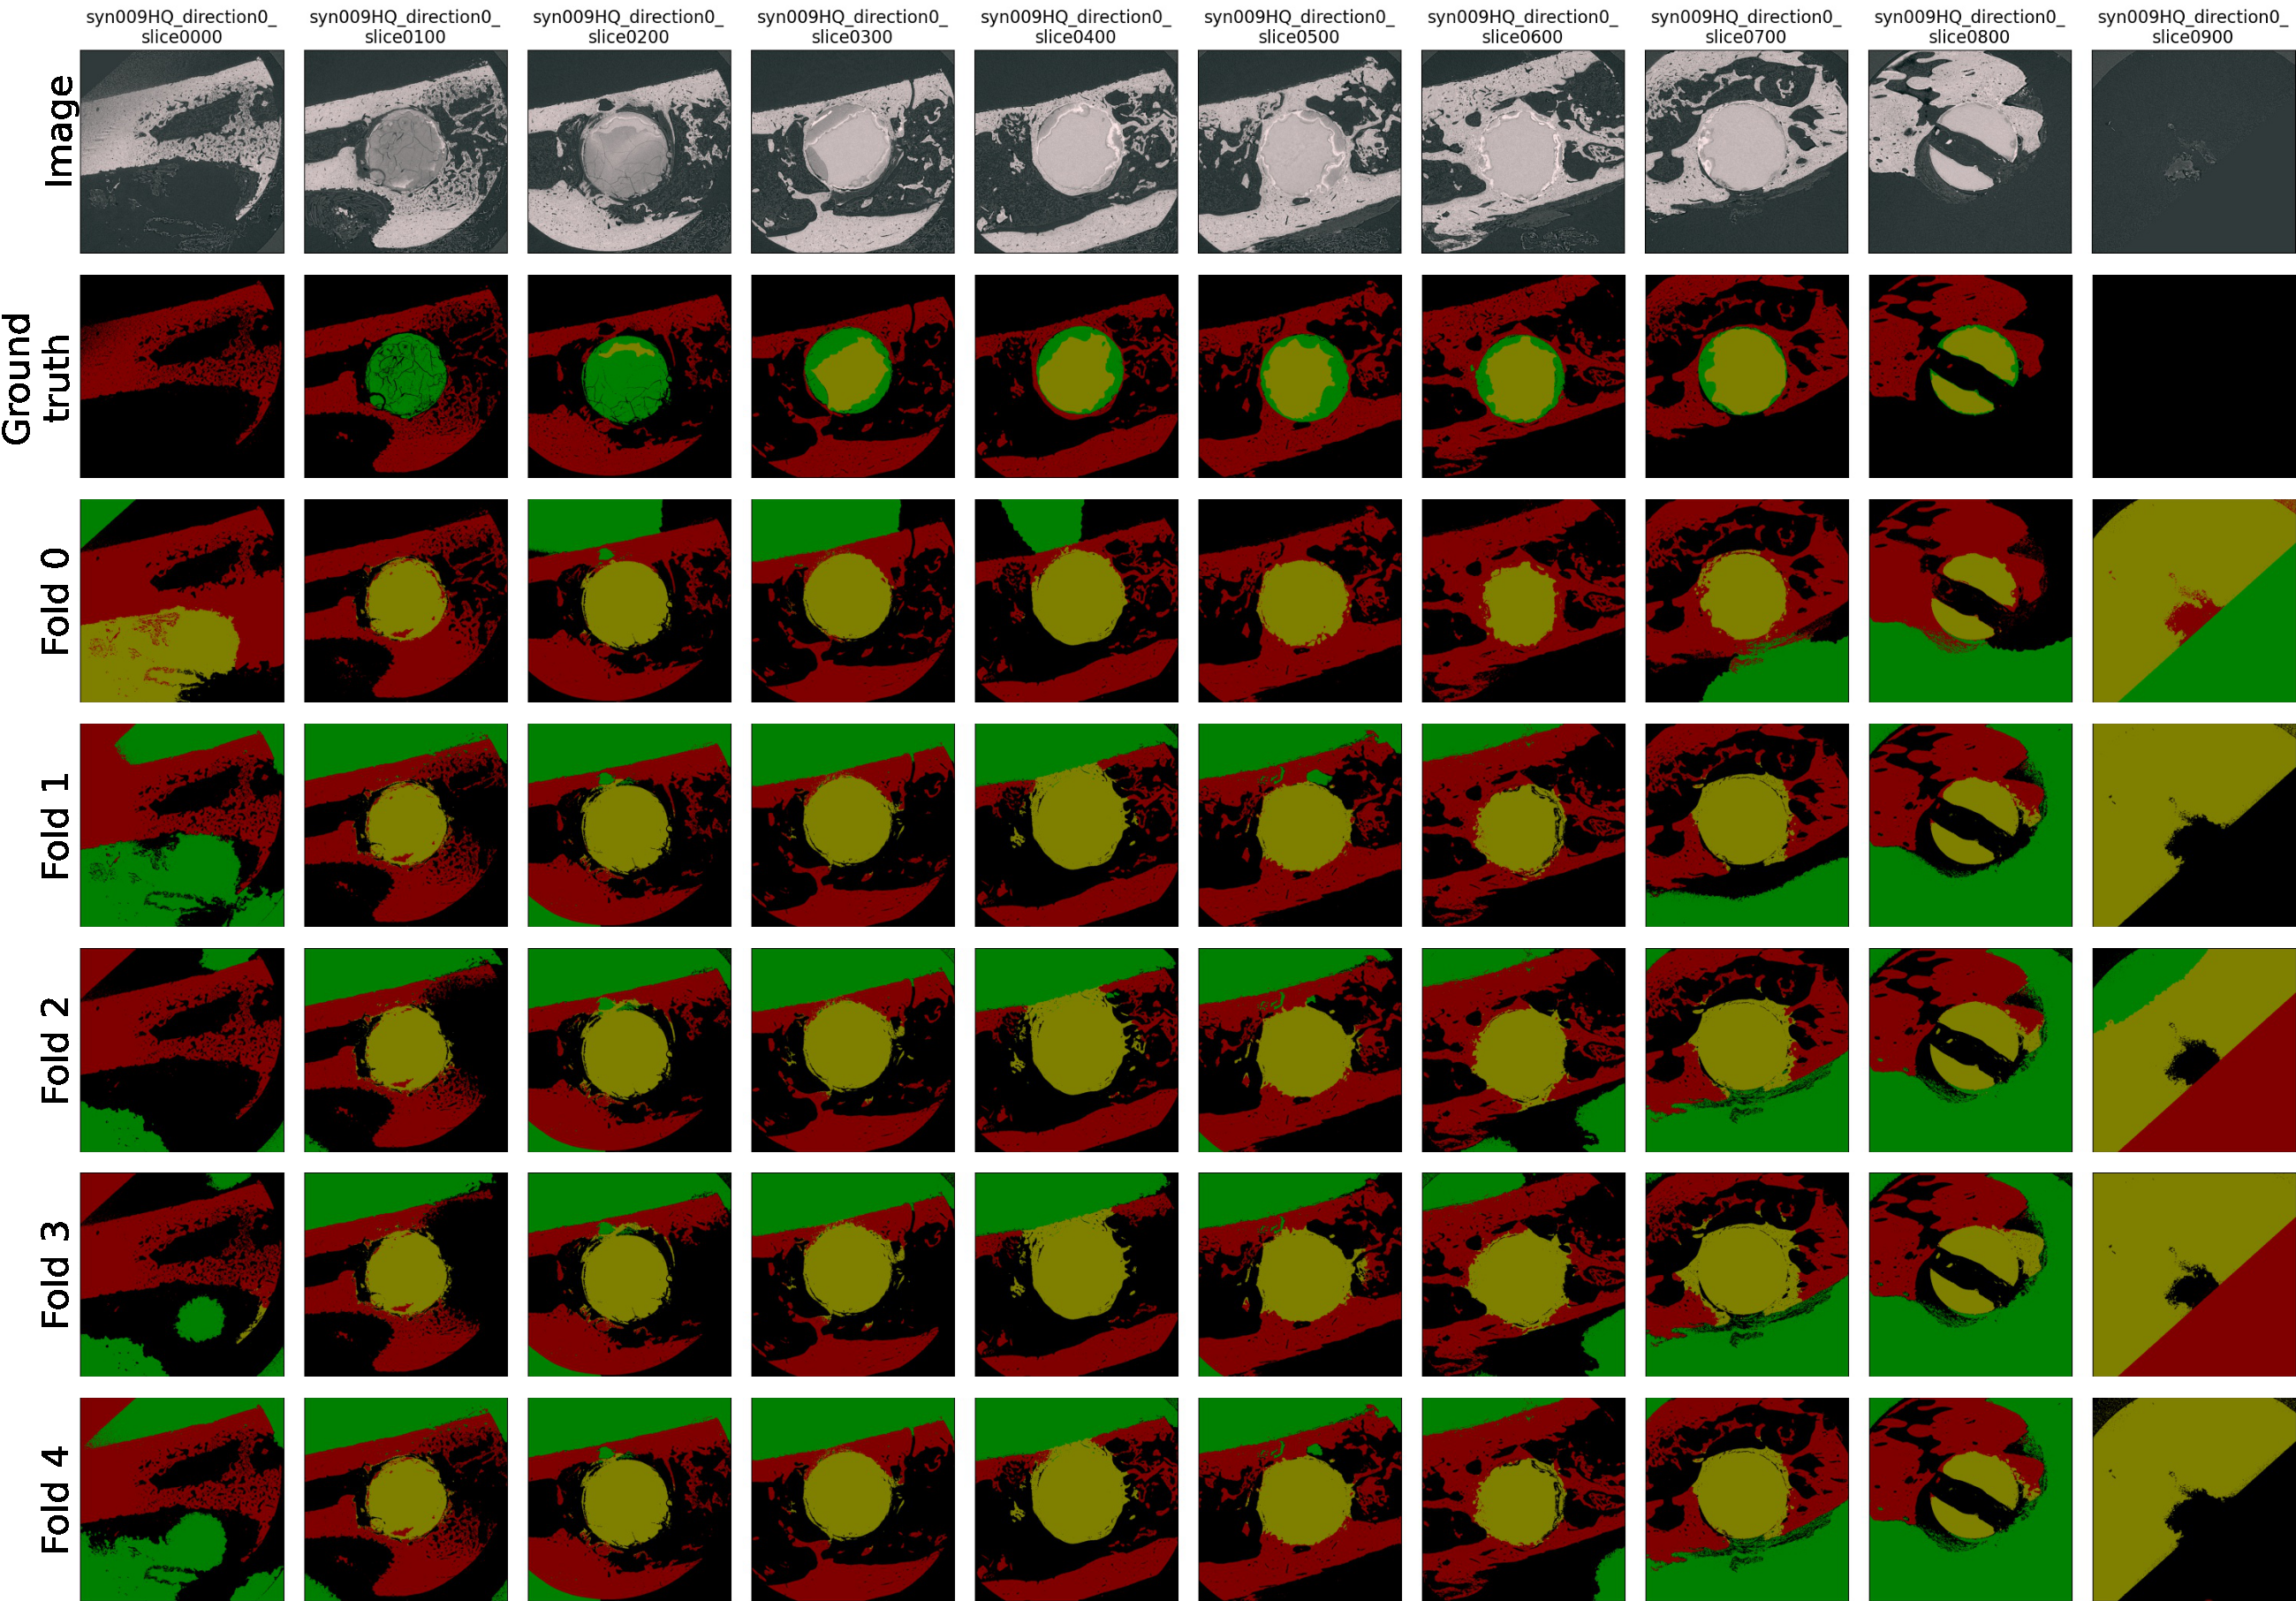
\includegraphics[clip,trim={0 0 0 7}, height=0.98\textwidth, angle=90]{pictures/experiment_2/base-case_final_example_predictions_2_all_folds}\\
    \caption[Predictions with Base Case]{Image, ground truth, and predictions of base-case (from each fold). Shown slices belong to volume syn009 (which was neither part of train nor validation set) and are ordered according to spatial location. Every 100th slice is shown. Image rotated by 90~degree.}
    \label{fig:base-case-predictions-syn009-by-fold}
\end{figure}

\clearpage
\begin{figure}[!htb]
    \centering
    %<left> <lower> <right> <upper>
    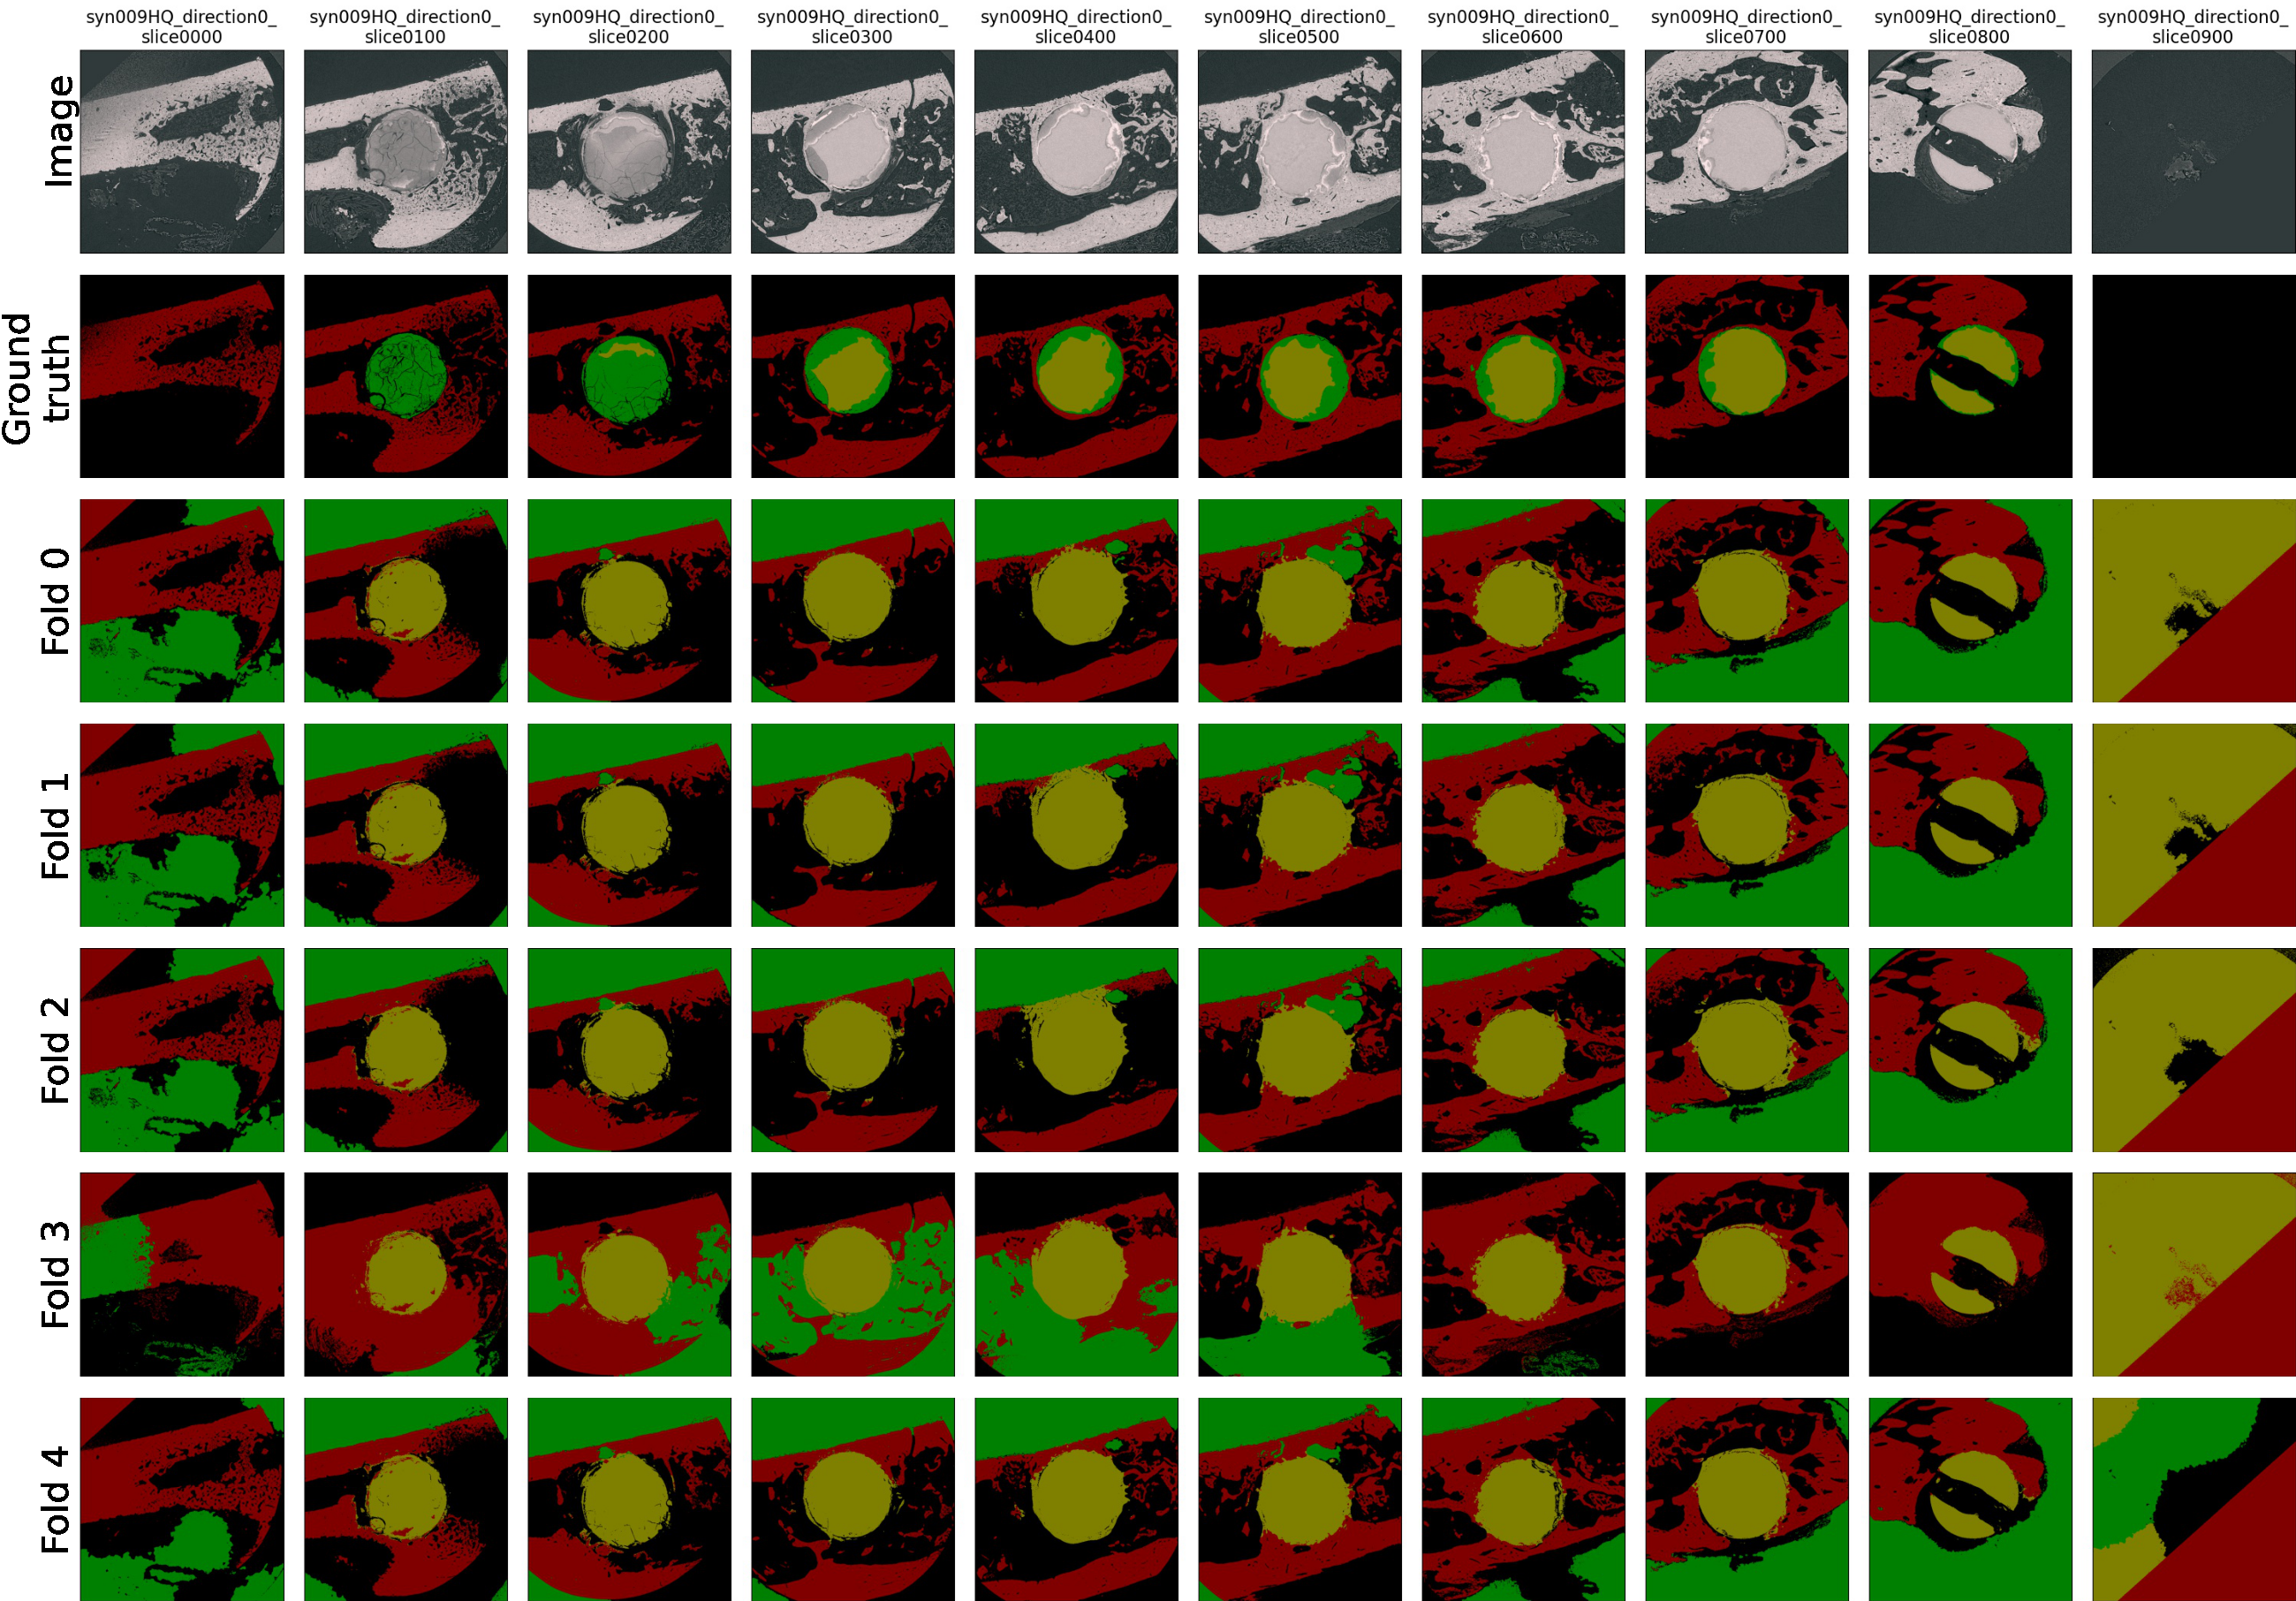
\includegraphics[clip,trim={0 0 0 7}, height=\textwidth, angle=90]{pictures/experiment_2/random_cropped_final_example_predictions_2_all_folds}\\
    \caption[Predictions with Random Cropped 200~px Regime]{Image, ground truth, and predictions of the random cropped 200~px model (from each fold).  Shown slices belong to volume syn009 (which was neither part of train nor validation set) and are ordered according to spatial location. Every 100th slice is shown. Image rotated by 90~degree.}
    \label{fig:random_cropped-predictions-syn009-by-fold}
\end{figure}

\clearpage
\begin{figure}[!htb]
    \centering
    %<left> <lower> <right> <upper>
    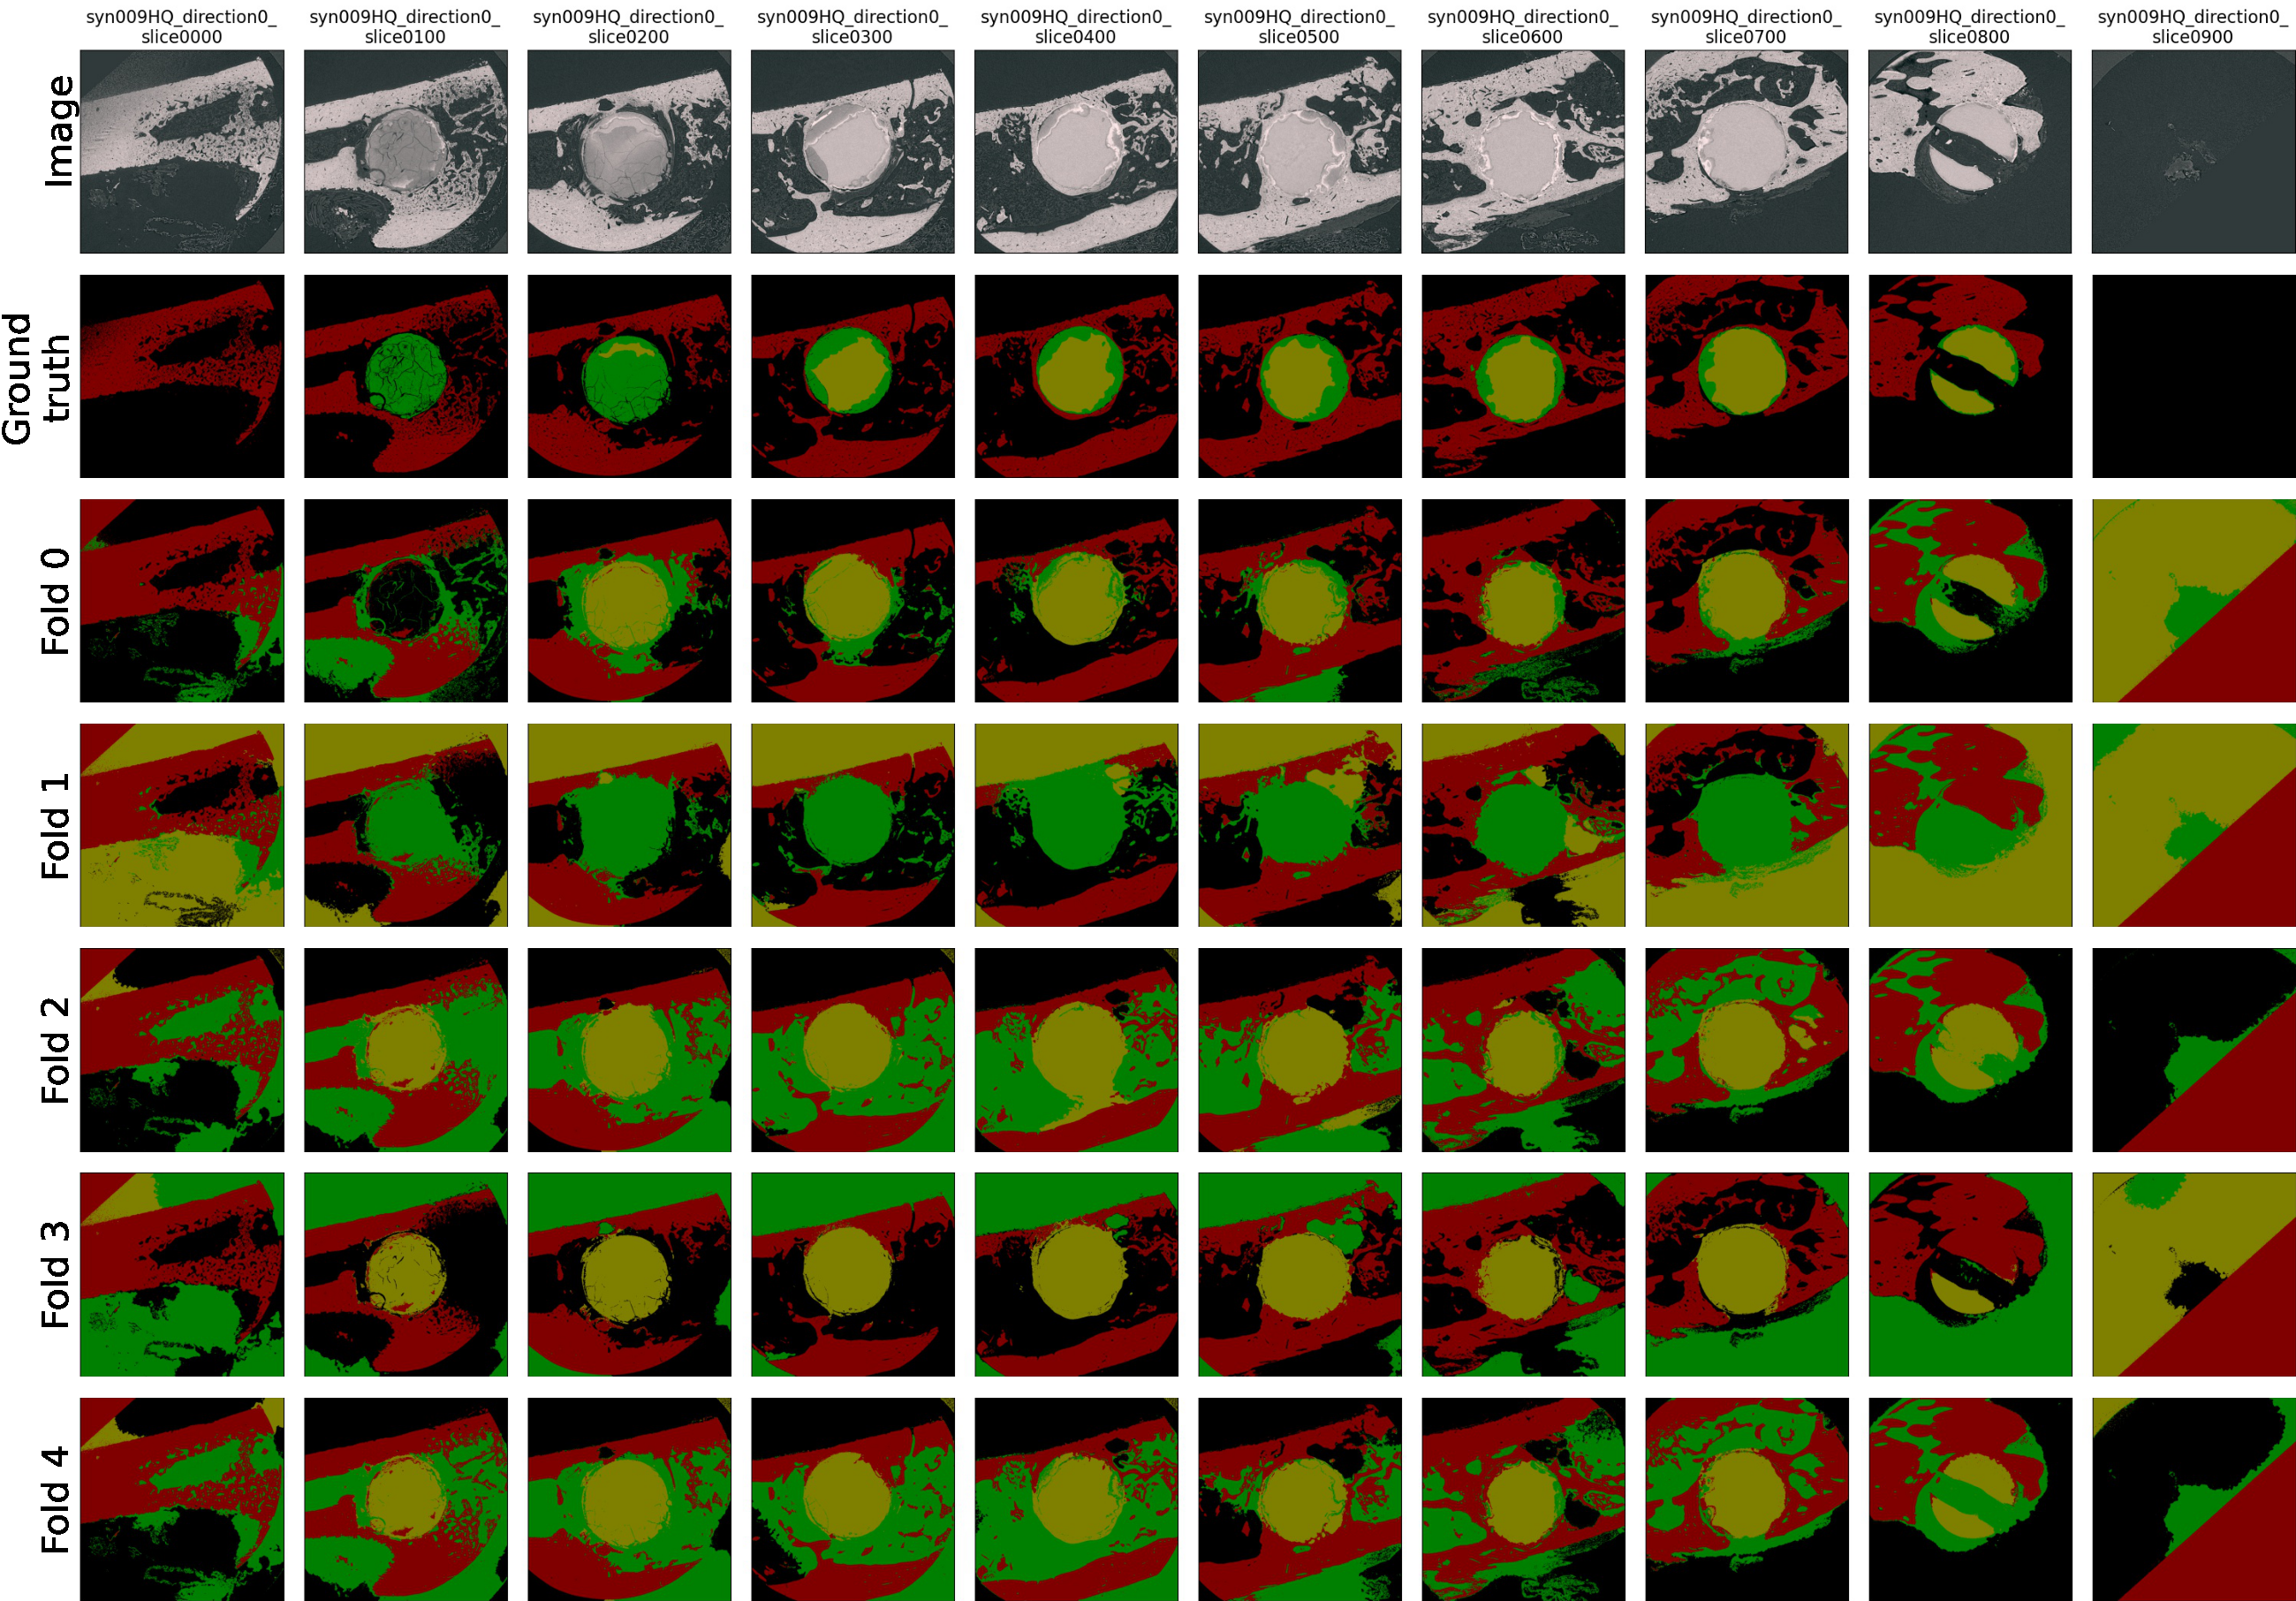
\includegraphics[clip,trim={0 0 0 7}, height=\textwidth, angle=90]{pictures/experiment_2/random_cropped_res96_final_example_predictions_2_all_folds}\\
    \caption[Predictions with Random Cropped 96~px Regime]{Image, ground truth, and predictions of the random cropped 96~px model (from each fold). Shown slices belong to volume syn009 (which was neither part of train nor validation set) and are ordered according to spatial location. Every 100th slice is shown. Image rotated by 90~degree.}
    \label{fig:random_cropped_96-predictions-syn009-by-fold}
\end{figure}

\clearpage
\begin{figure}[!htb]
    \centering
    %<left> <lower> <right> <upper>
    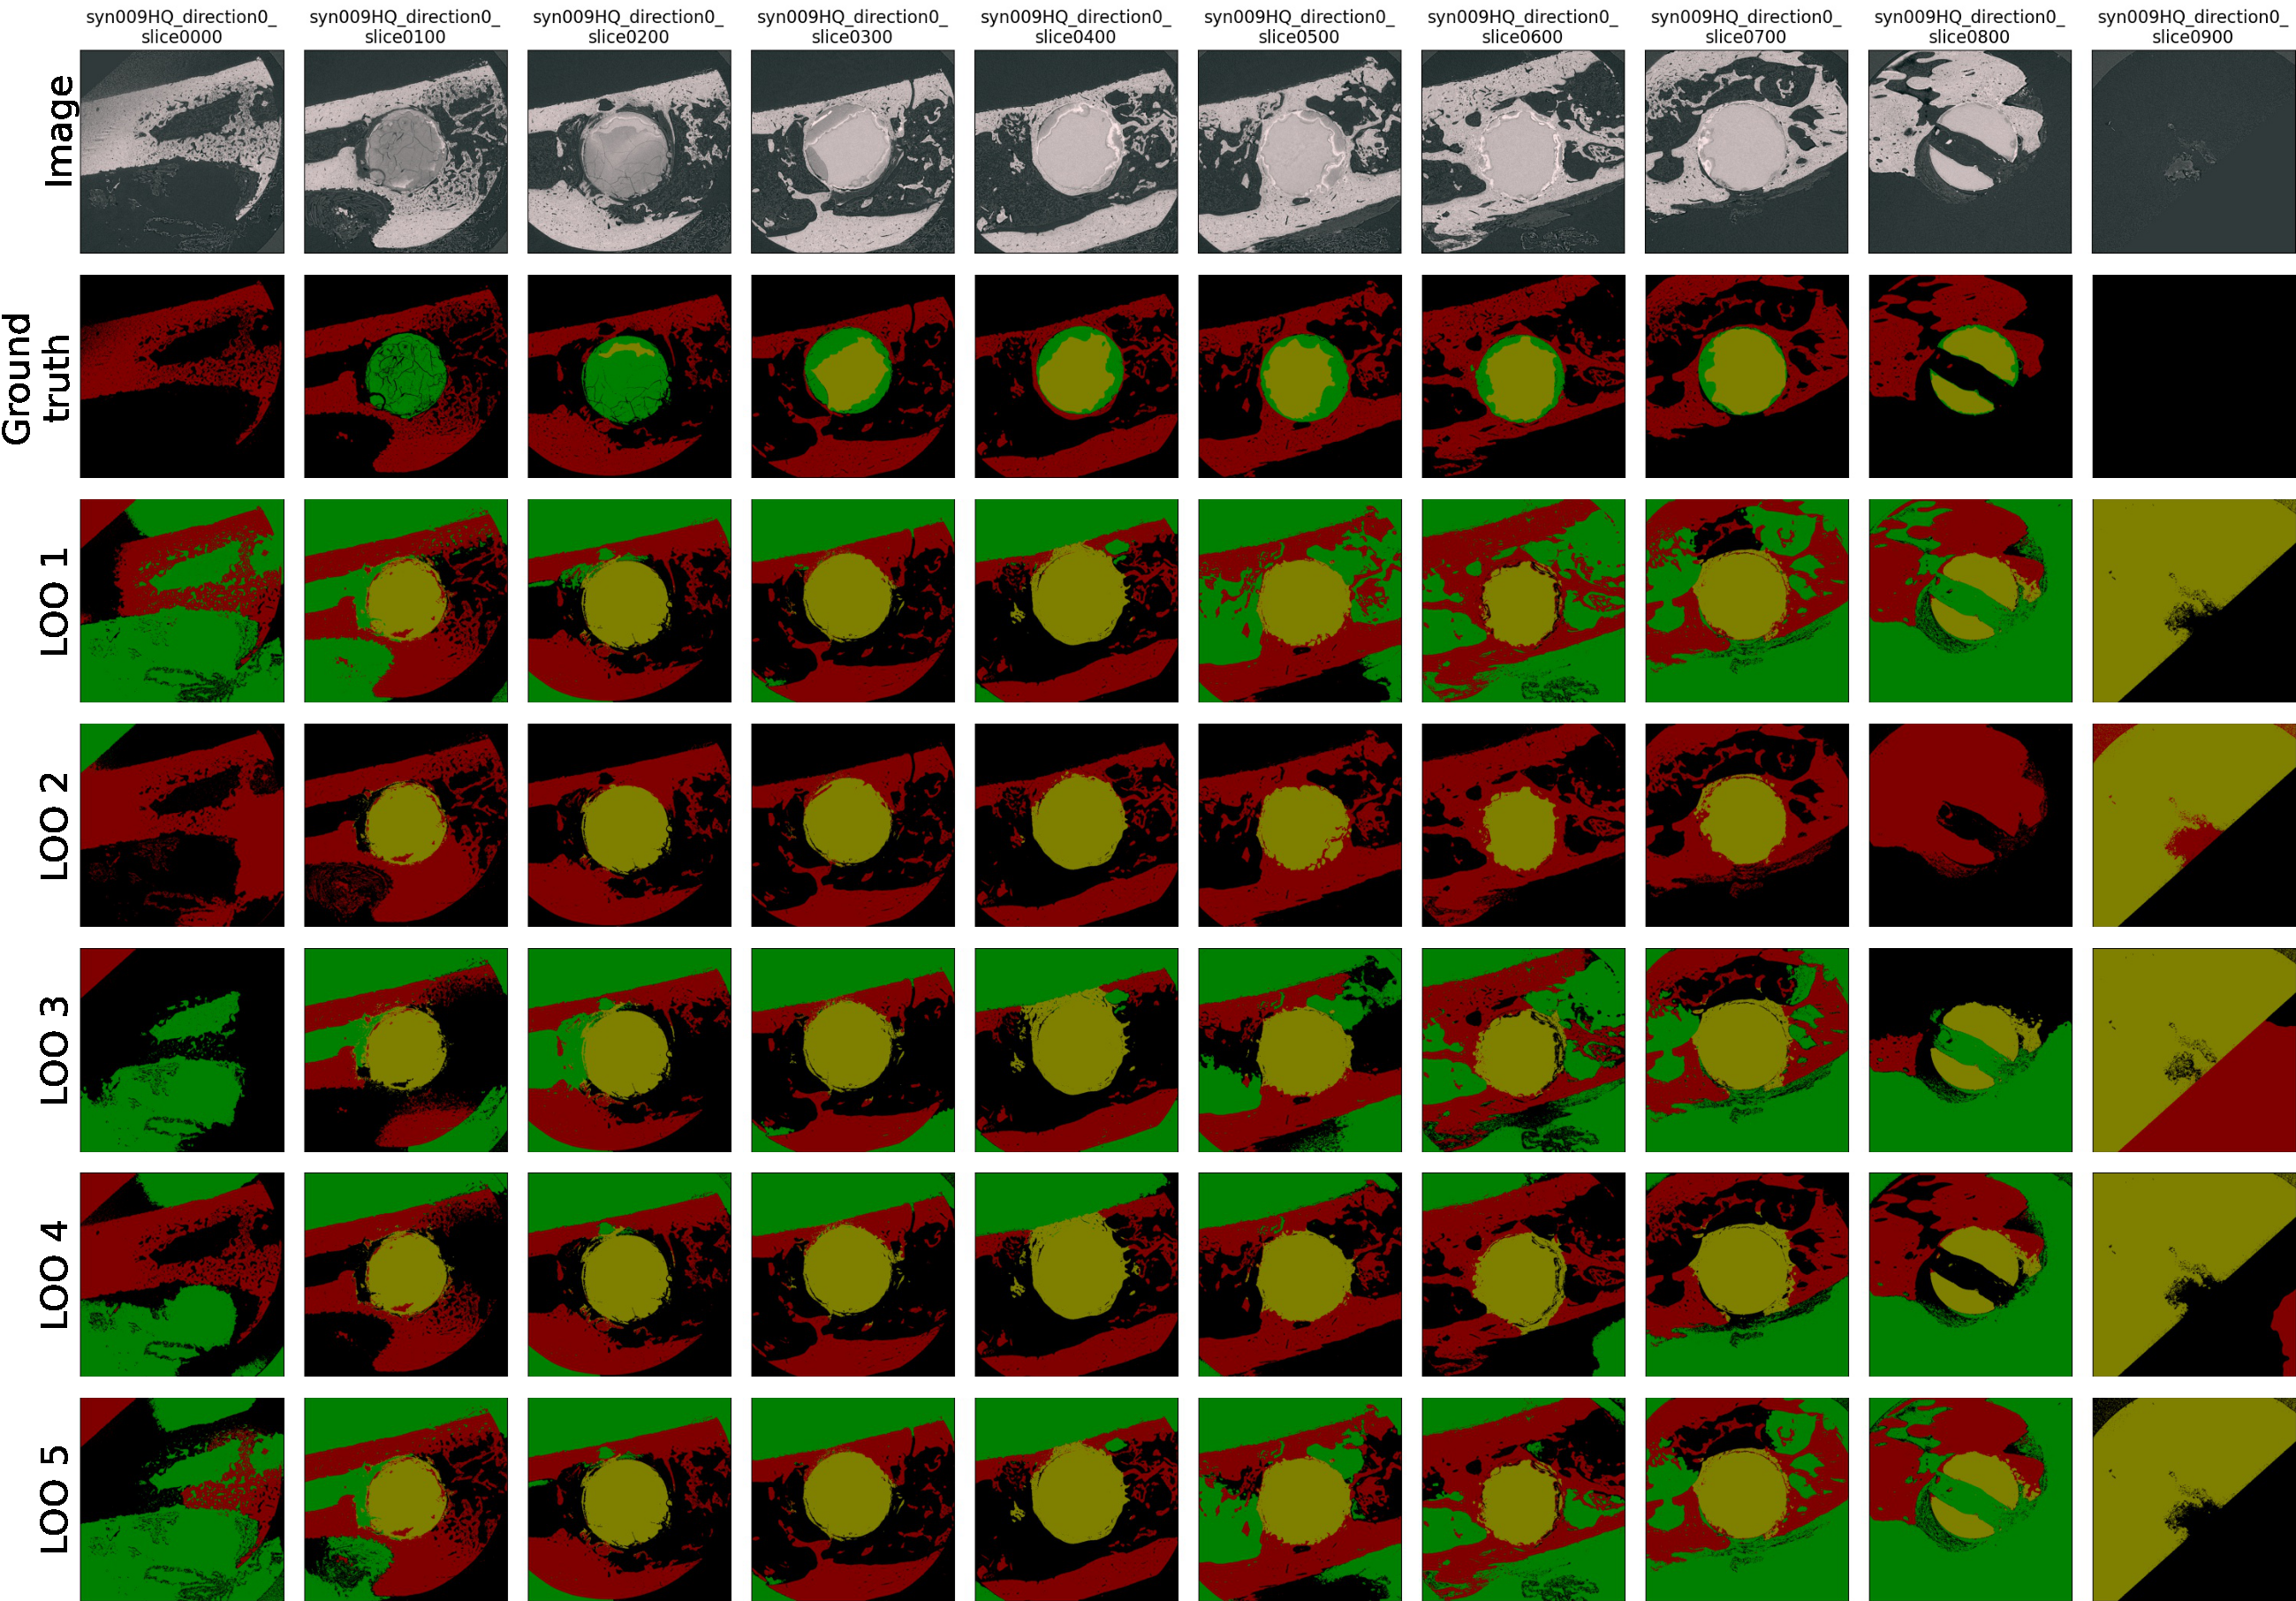
\includegraphics[clip,trim={0 0 0 7}, height=\textwidth, angle=90]{pictures/experiment_2/base-case_LOO_example_predictions_2_all_folds}\\
    \caption[Predictions with Leave-one-out Cross-validation]{Image, ground truth, and predictions of the leave-one-out cross-validation model (from each fold). Shown slices belong to volume syn009 (which was neither part of train nor validation set) and are ordered according to spatial location. Every 100th slice is shown. Image rotated by 90~degree.}
    \label{fig:loo-predictions-syn009-by-fold}
\end{figure}

\clearpage
\begin{figure}[!htb]
    \centering
    %<left> <lower> <right> <upper>
    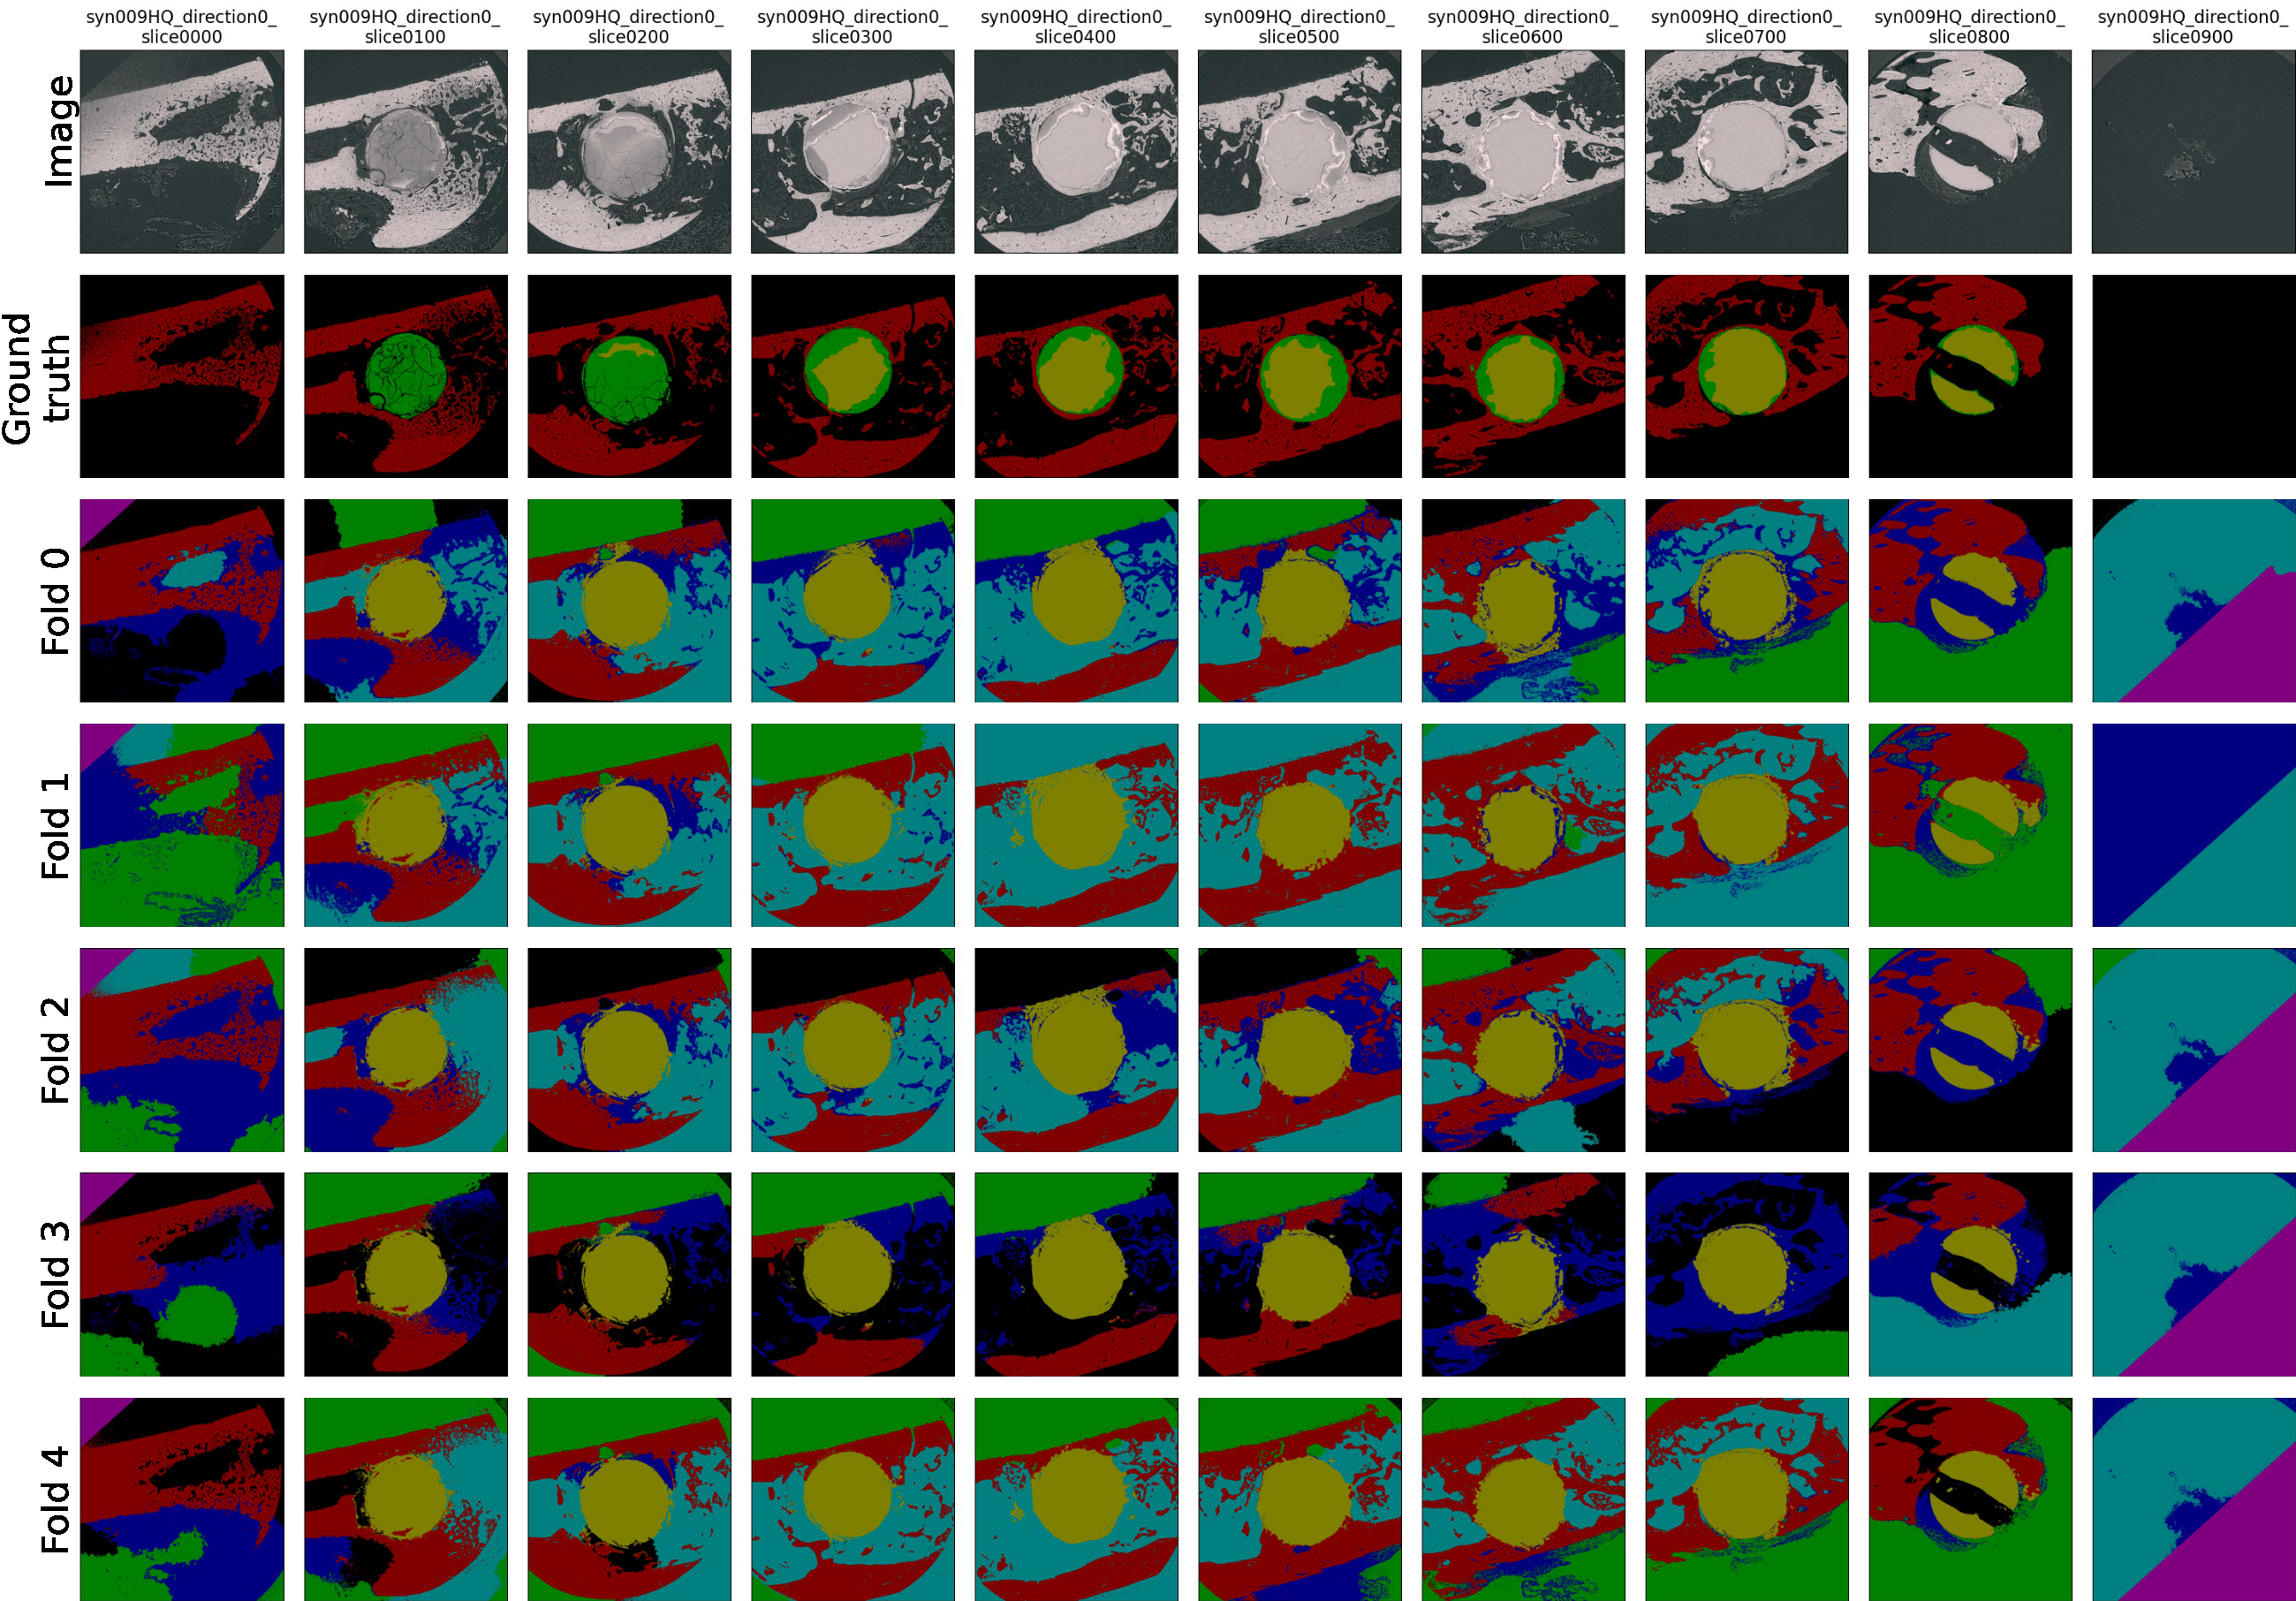
\includegraphics[clip,trim={0 0 0 7}, height=\textwidth, angle=90]{pictures/experiment_2/extra_clusters3_example_predictions_2_all_folds}\\
    \caption[Predictions with Three Extra Clusters]{Image, ground truth, and predictions of the model trained with 3 extra clusters (predictions from each fold). Shown slices belong to volume syn009 (which was neither part of train nor validation set) and are ordered according to spatial location. Every 100th slice is shown. Image rotated by 90~degree.}
    \label{fig:extra_clusters3-predictions-syn009-by-fold}
\end{figure}

\clearpage
\begin{figure}[!htb]
    \centering
    %<left> <lower> <right> <upper>
    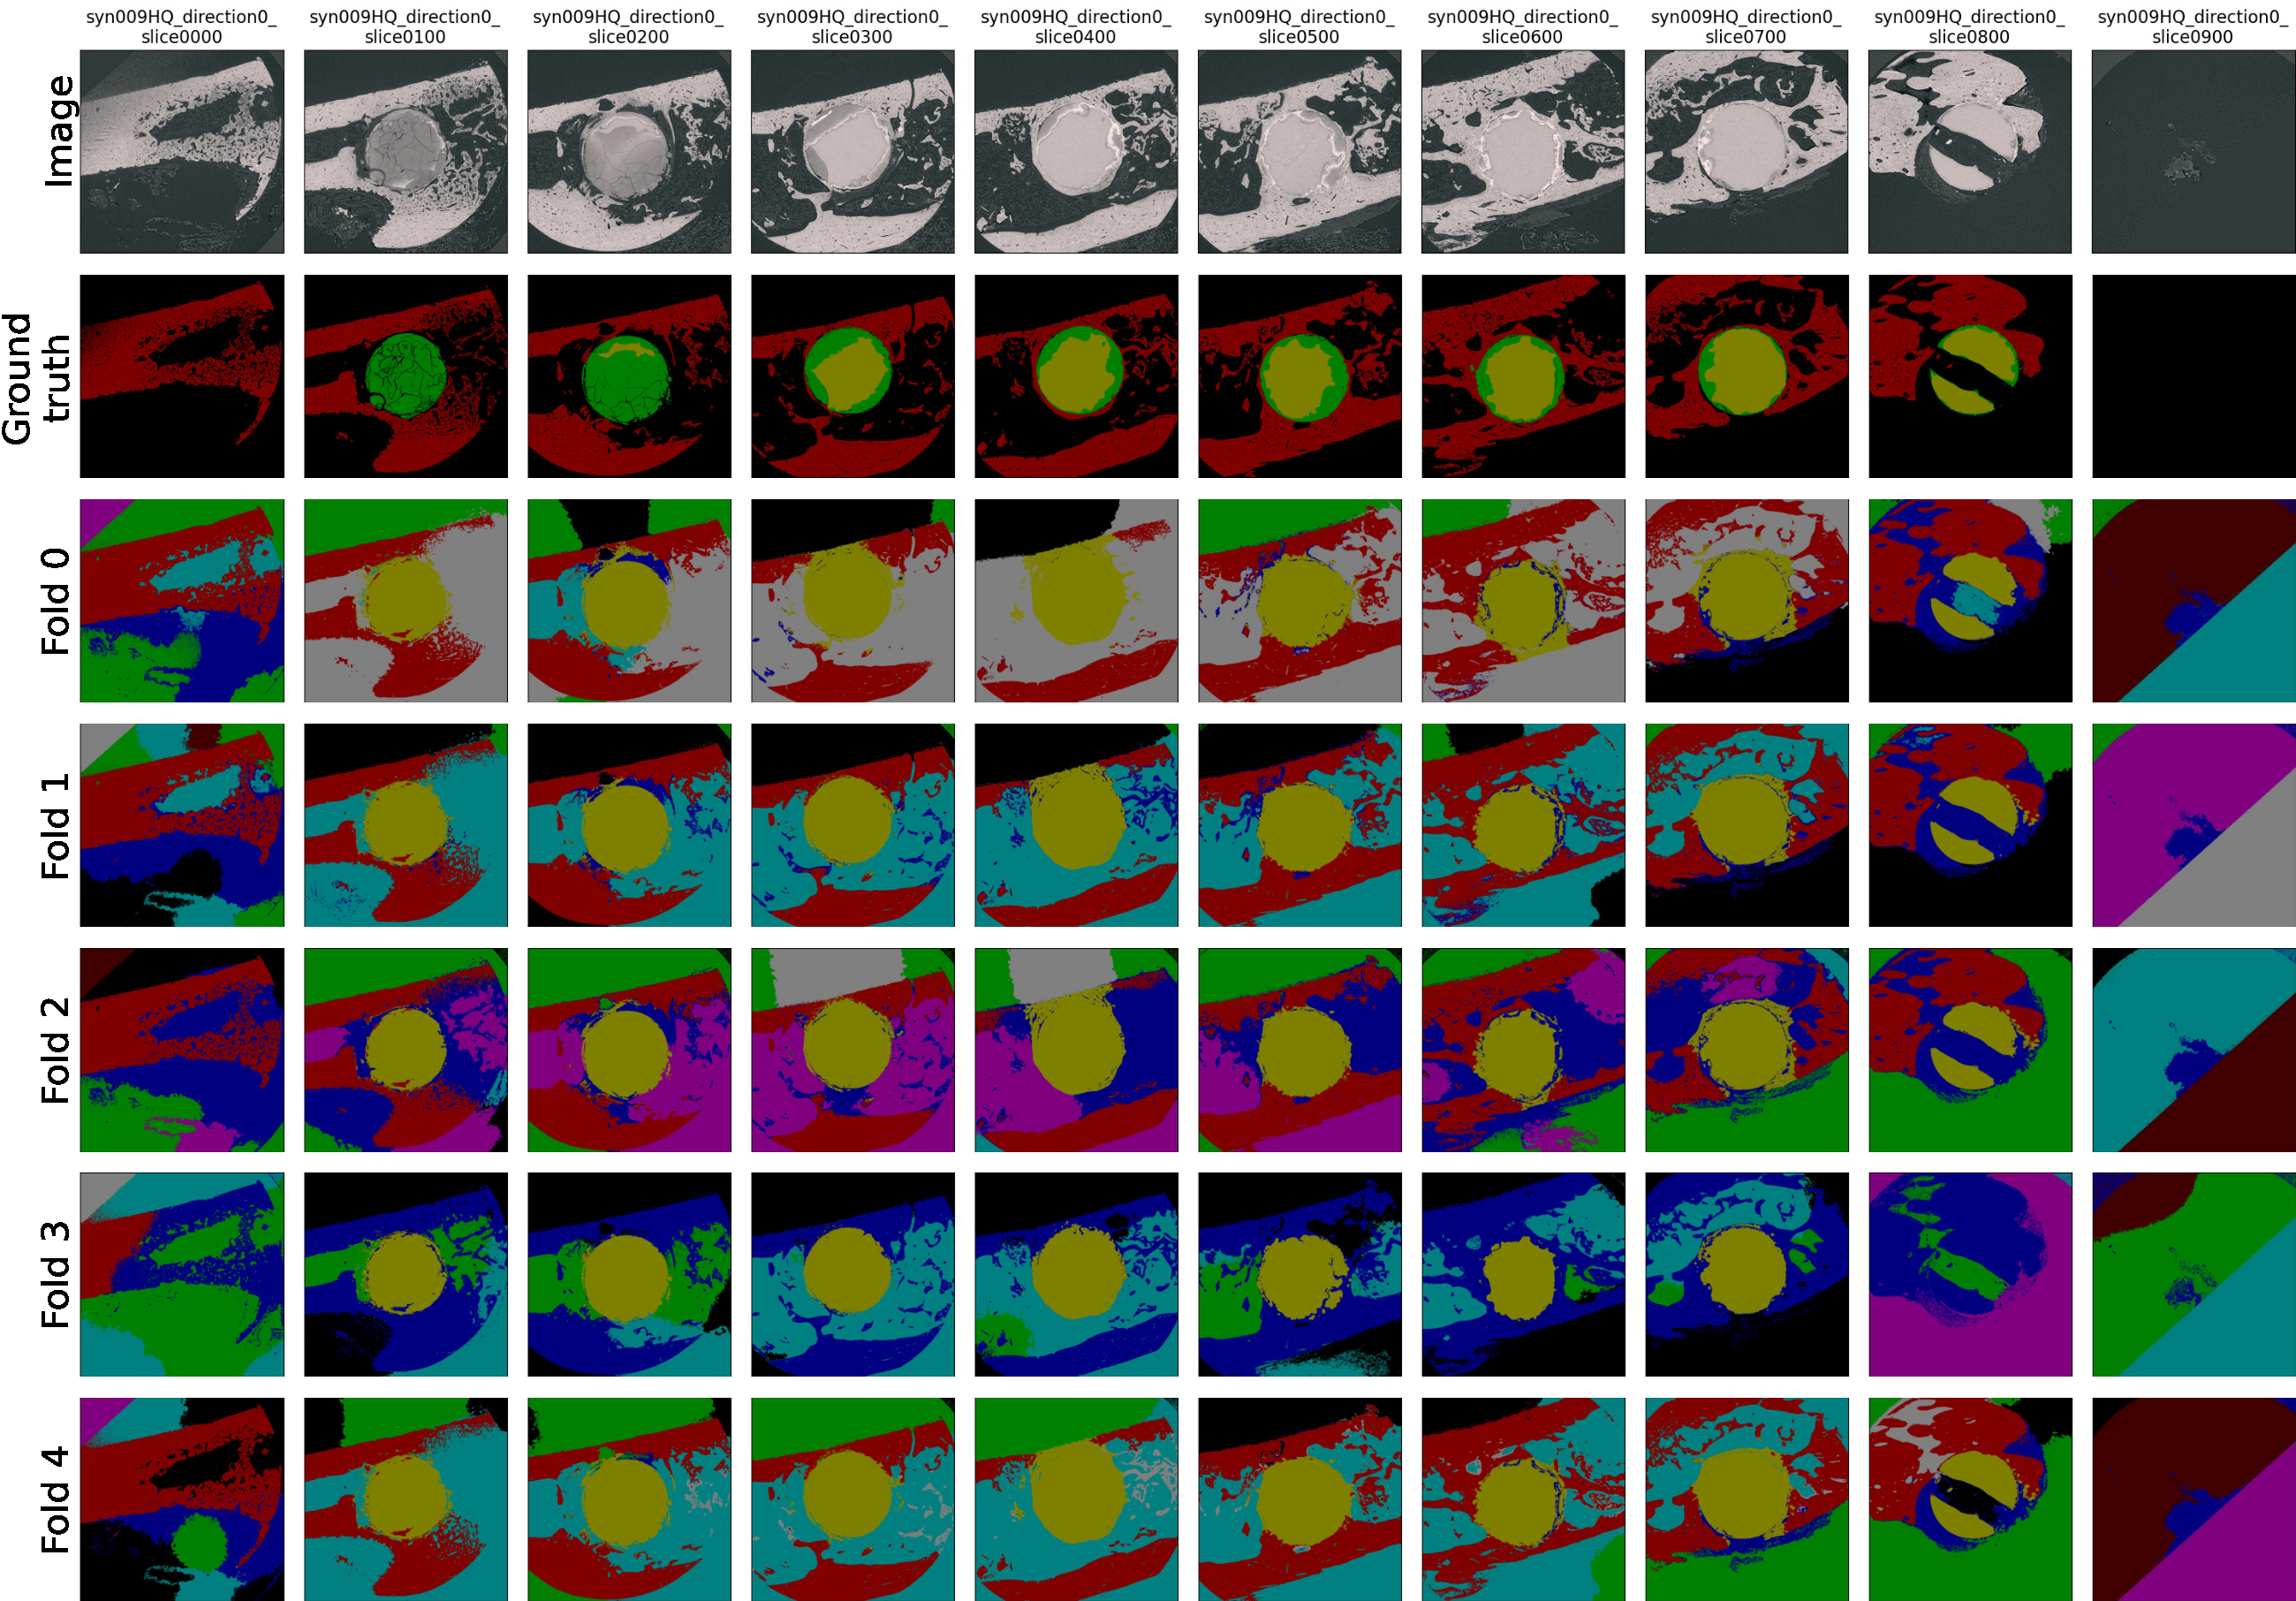
\includegraphics[clip,trim={0 0 0 7}, height=\textwidth, angle=90]{pictures/experiment_2/extra_clusters5_example_predictions_2_all_folds}\\
    \caption[Predictions with Five Extra Clusters]{Image, ground truth, and predictions of the model trained with 5 extra clusters (predictions from each fold). Shown slices belong to volume syn009 (which was neither part of train nor validation set) and are ordered according to spatial location. Every 100th slice is shown. Image rotated by 90~degree.}
    \label{fig:extra_clusters5-predictions-syn009-by-fold}
\end{figure}

\clearpage
\begin{figure}[!htb]
    \centering
    %<left> <lower> <right> <upper>
    \includegraphics[clip,trim={0 0 0 7}, height=\textwidth, angle=90]{pictures/experiment_2/extra_clusters10_example_predictions_2_all_folds}\\
    \caption[Predictions with Ten Extra Clusters]{Image, ground truth, and predictions of the model trained with 10 extra clusters (predictions from each fold). Shown slices belong to volume syn009 (which was neither part of train nor validation set) and are ordered according to spatial location. Every 100th slice is shown. Image rotated by 90~degree.}
    \label{fig:extra_clusters10-predictions-syn009-by-fold}
\end{figure}
